\section{Resultados modelo base MD2}
\label{sec:resultados_modelo_base}

A continuación se presentan los resultados obtenidos en \todo{cita Damián} del Modelo de TRFs por Regresión Regularizada en el modelo MD2 presentado en la sección \ref{sec:modelo_regresion}. Como paso previo a 
la incorporación de las features del nnELM, se replicó el modelo MD2 sobre el 
dataset HSEM siguiendo la metodología descripta en la Sección~\ref{sec:modelo_regresion}. 
Los resultados obtenidos son consistentes con los reportados en \todo{cita Damián}, 
lo que valida el pipeline de análisis y establece la línea de base sobre la cual 
se evaluará la contribución de cada experimento.

La Figura~\ref{fig:modelo_base} presenta las TRFs grupales y los clusters 
significativos según TFCE para cada predictor del modelo MD2.

\begin{figure}[H]
    \centering
    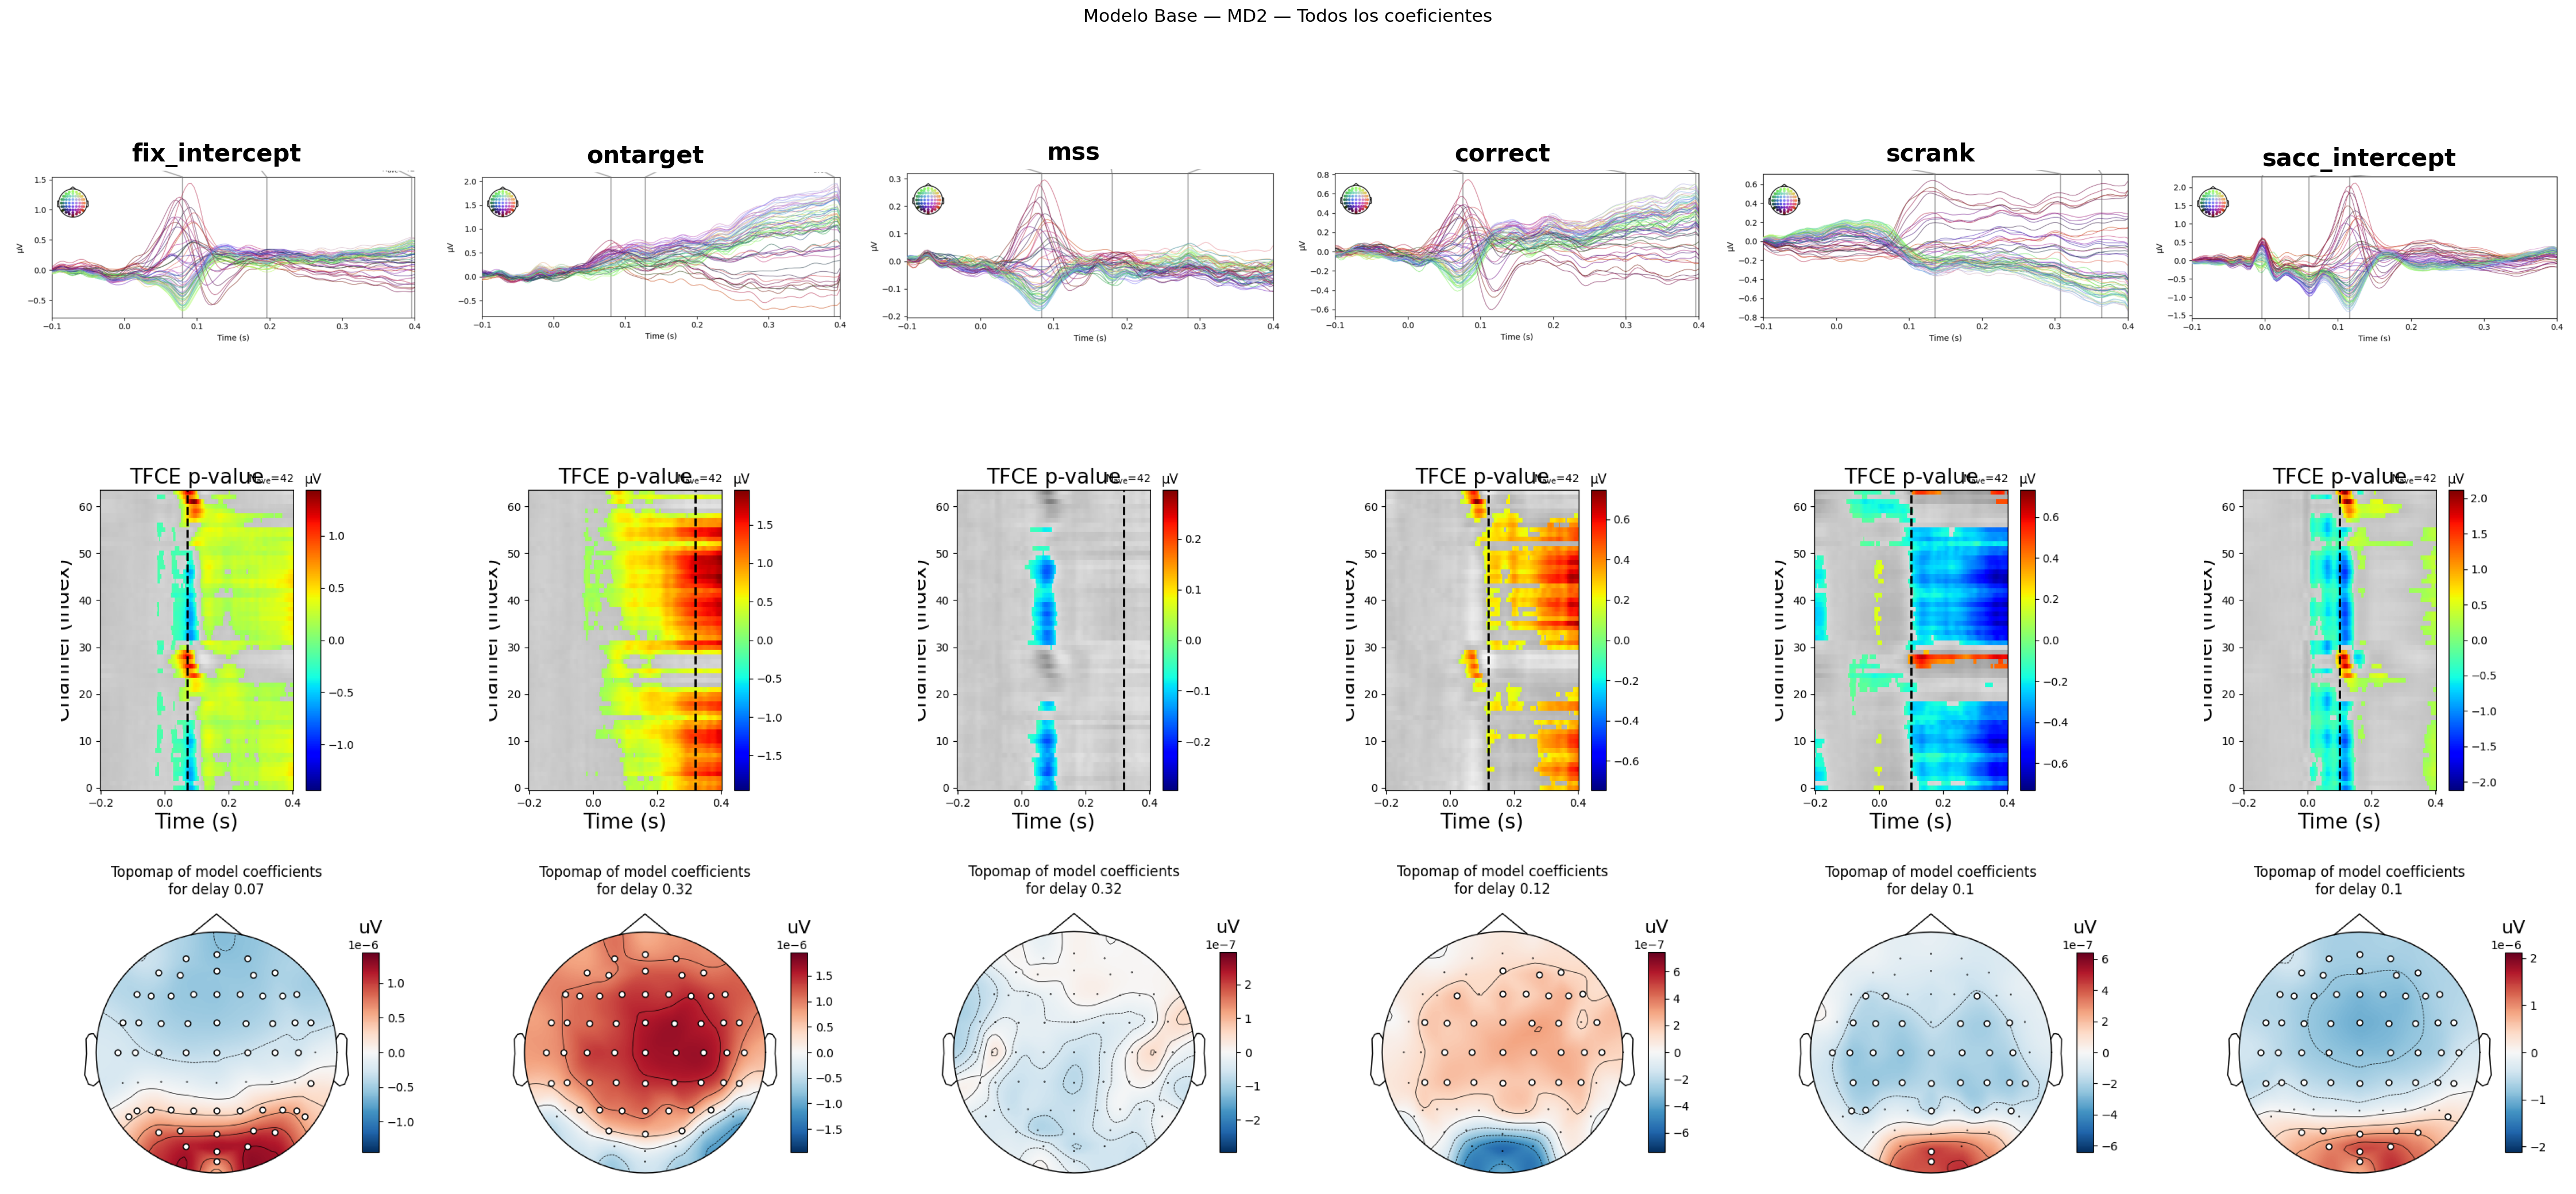
\includegraphics[width=\textwidth]{chapters/04_resultados/images/modelo_base_todos_coeffs}
    \caption{Resultados del modelo base guiado por hipótesis (MD2). Para cada predictor se muestra: (fila superior) el curso temporal de las estimaciones (TRFs) para todos los electrodos, con las cabezas topográficas indicando la distribución espacial en los picos de actividad; (fila media) el mapa espacio-temporal de los coeficientes, enmascarado por los clústeres significativos según la prueba estadística TFCE (N=42); y (fila inferior) la topografía de los coeficientes en el instante de máxima actividad (marcado por las líneas punteadas verticales), donde los círculos blancos resaltan los electrodos específicos que forman parte del clúster significativo.}
    \label{fig:modelo_base}
\end{figure}


La Figura~\ref{fig:modelo_base} presenta las TRFs grupales y los clusters 
significativos según TFCE para cada predictor del modelo MD2. Las estimaciones de las TRFs reportadas por los autores de cada variable incluyen los siguientes efectos principales:

\textbf{Intercept de fijación.} Esta variable captura la respuesta base del cerebro cada vez que los ojos se posan sobre cualquier estímulo. Se revela una activación temprana que activa su pico a los ~78 ms, mostrando un clúster significativo según la prueba TFCE con actividad positiva en la región occipital y negativa en la región fronto-central. Esta latencia y distribución espacial son consistentes con el componente visual P100.

\textbf{Target (ontarget).} Las fijaciones que cayeron sobre un objetivo generaron activaciones generalizadas en un clúster significativo que abarcó electrodos centrales, frontales, temporales y parietales. Se observó un aumento de la actividad alrededor de los 300ms, un patrón que se alinea con el componente P300 asociado a la detección de objetos y al procesamiento cognitivo consciente.

\textbf{Memory Set Size (MSS).}  La manipulación de la carga de memoria demostró activar respuestas visuales tempranas. Se identificó un cluster significativo con activaciones fronto-centrales a los 78ms, indicando una respuesta negativa de la amplitud del componente P100 a medida que aumenta la carga de memoria. En el contexto de la búsqueda híbrida, este efecto se interpreta como un aumento del control cognitivo interno (top down).

\textbf{Correct.} La variable categórica que codifica si el ensayo terminó en una respuesta correcta mostró un efecto principal estable y robusto al ser introducida en el modelo.

\textbf{Scrank (TPS).} Denominado Task Progress Score (TPS), este predictor modelo el rango estandarizado de la fijación para capturar el progreso temporal del ensayo. Su inclusión reveló un clúster significativo sobre la región occipital, que se mantiene consistente a lo largo de toda la ventana de la fijación. Este efecto sostenido sugiere una activación continua de las predicciones del sujeto y una evaluación constante de la evidencia visual acumulada a medida que avanza la búsqueda.

\textbf{Intercept de sacada.} Predictor que aisla la actividad generada puramente por la ejecución del movimiento ocular. Mostró activaciones robustas con un pico alrededor de los 120ms, consistentes con la respuesta lambda.